% --------------------------------------------------------------
% This is all preamble
% --------------------------------------------------------------
 
\documentclass[10pt]{article}


% Basic Packages for Encoding (Input AND Output) and Langauge Support
\usepackage[utf8]{inputenc}
\usepackage[T1]{fontenc}
\usepackage[french]{babel}

% Change Layout with a User-Friendly Interface
\usepackage[margin=1in]{geometry} 

% Include Pictures with a User-Friendly Interface
\usepackage{graphicx}
\graphicspath{ {./images/calculus/} }
\usepackage{float}

% Extended Math Support from the Famous 'American Mathematical Society'
\usepackage{amsmath,amsthm,amssymb}

% Section title formatting
\usepackage{titlesec}

\titleformat{\section}
            {\normalfont\scshape}{\thesection}{1em}{}

\newcommand{\N}{\mathbb{N}}
\newcommand{\Z}{\mathbb{Z}}

\usepackage{pgfplots}


%Numbered Questions 
\newcounter{question}
\newenvironment{question}
               {\refstepcounter{question}\par\medskip\noindent\textbf{Q~\thequestion.}\par \noindent \rmfamily}
               {\medskip}

\begin{document}
 
% --------------------------------------------------------------
%                        Actual content
% --------------------------------------------------------------

\title{Exercices de révision: Calcul}
\author{Annie B. \thanks{Les questions sont tirées des examens de l’IB de 2018, 2012, 2011, 2010, 2007}}
\date{\today}
\maketitle

\section*{\textbf{Calculatrice Graphique Non Permise}}
%1
\begin{question}
  \hspace*{\fill} [Note maximale: 6]\par
  \noindent Soit la fonction $f(x) = 6x^2-3x$ representé ci-dessous\par
  \medskip

  %
  % Plot begins
  %
  \scalebox{.5}[1.0]{ % {horizontal scale} [vertical scale]
  \begin{tikzpicture}
  \begin{axis}[
    xlabel=$x$,
    ylabel=$f(x)$
    ] 
    \addplot [xscale=1.0, yscale=1.0, smooth] coordinates{(0, 0) (0,20)}; % y axis
    \addplot [xscale=1.0, yscale=1.0, domain=0:2.2, smooth] { 0 }; % x axis
    \addplot [xscale=1.0, yscale=1.0, smooth] coordinates{ (1,0) (1, 3) }; 
    \addplot [xscale=1.0, yscale=1.0, smooth] coordinates{ (2,0) (2, 18) };
    \addplot [xscale=1.0, yscale=1.0, domain=0:2.2, smooth] { 6 * x^2 - 3*x }; % f(x)
  \end{axis}
  \end{tikzpicture}}\par
  %
  % Plot ends
  %
  \medskip
  (a) Trouvez $\int \! (6x^2-3x) \, \mathrm{d}x$\hspace*{\fill} [2]\par
  \medskip

  (b) Trouvez l’aire de la région délimitée par la représentation graphique de $f(x)$,\par
  \hspace{1em} l’axe des abscisses et les droites x = 1 et x = 2.\par
  \hspace{1em} C'est à dire $\int_1^2 \! (6x^2-3x) \, \mathrm{d}x$ \hspace*{\fill} [4]

\end{question}

\newpage
%2
\begin{question}
  \hspace*{\fill} [Note maximale: 15]\par
  \noindent Une boîte en métal, cylindrique et fermée, de rayon égal à $r$ centimètres et de hauteur égale à $h$ centimètres possède un volume de $20\pi$ $cm^3$.\par
  
  \medskip
  \begin{flushleft}
    \noindent La figure n'est pas a l'échelle\par
    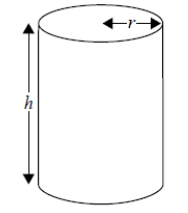
\includegraphics[scale=0.5]{cylindre.png}\par
  \end{flushleft}
  \medskip

  (a) Exprimez $h$ en fonction de $r$.\hspace*{\fill} [2]\par
  \medskip
  \noindent Le métal pour la base et le couvercle de la boîte coûte 10 cents le $cm^2$ et le métal pour le côté incurvé coûte 8 cents le $cm^2$. Le coût total du métal, en cents, est de $C$.\par
  \medskip
  (b) Montrez que $C$ $=$ $20\pi{}r^2 + \frac{320\pi}{r}$\hspace*{\fill} [4]\par
  \medskip

  (c) Sachant qu’il existe une valeur minimale pour $C$, trouvez cette valeur minimale en fonction de $\pi$ \hspace*{\fill} [9]\par
\end{question}

\bigskip
%3
\begin{question}
  \hspace*{\fill} [Note maximale: 16]\par

  \noindent Considérez une fonction $f(x)$. la droite $L_1$ d’équation $y = 3x + 1$ est une tangente à la représentation graphique de $f(x)$ lorsque $x = 2$.\par
  \medskip
  (a)\par
  \hspace{2em} (i)  Écrivez $f^\prime(2)$.\par
  \medskip
  \hspace{2em} (ii) Trouvez $f(2)$.\hspace*{\fill} [4]\par
  \medskip
  \noindent Soit $g(x) = f(x^2 + 1)$ et $P$ le point sur la représentation graphique de $g$ où $x = 1$\par
  \medskip
  (b) Montrez que la représentation graphique de $g$ a une pente de 6 au point $P$.\hspace*{\fill} [5]\par
  \medskip
  (c) Soit $L_2$ la tangente à la représentation graphique de $g$ au point $P$. $L_1$ coupe $L_2$ au point $Q$.\par
  \hspace{1em} Trouvez l’ordonnée de $Q$.\hspace*{\fill} [7]\par
\end{question}
\newpage
%4
\begin{question}
  \hspace*{\fill} [Note maximale: 15]\par
  \medskip
  \noindent La figure suivante donne la représentation graphique de $f(x) = a\,Cos\,bx $, pour $ 0 \le x \le 4$.\par  
  \medskip
  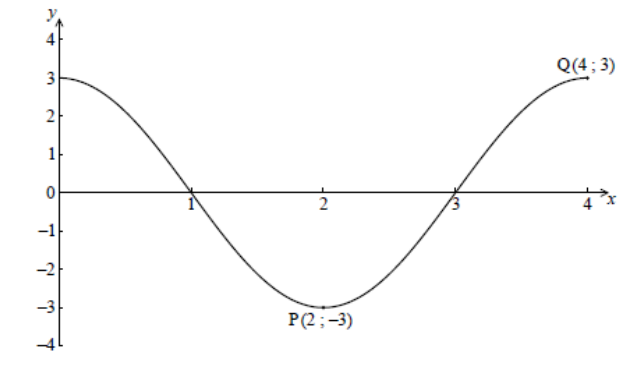
\includegraphics[scale=0.3]{temp_cos_wave}\par
  \medskip
  \noindent Il y a un point minimum en $P$ ( 2, -3 ) et un point maximum en $Q$ (4, 3).\par
  \medskip
  (a)\par
  \hspace{1em} (i)  Donnez la valeur de $a$.\par
  \medskip
  \hspace{1em} (ii) Trouvez la valeur de $b$.\hspace*{\fill} [3]\par
  \medskip
  (b) Donnez la pente de la courbe en P.\hspace*{\fill} [1]\par
  \medskip
  (c) Donnez l’équation de la normale à la courbe en P.\hspace*{\fill} [2]\par
  \medskip
\end{question}
\bigskip
%5
\begin{question}
  \hspace*{\fill} [Note maximale: 6]\par
  \medskip
  \noindent Soit $h(x) = \frac{6x}{cos x}.$\par
  \medskip
  Trouvez $h^\prime(0)$.\hspace*{\fill} [6]\par
\end{question}

%6
\bigskip
\begin{question}
  \hspace*{\fill} [Note maximale: 16]\par
  \medskip
  \noindent La figure suivante représente une partie de la représentation graphique de $f(x) = 2x\sqrt[2]{a^2 - x^2}$,\par
  \noindent pour $-1 \le x \le a$, où $a > 1$\par
  \begin{center}
    \noindent La figure n'est pas a l'échelle\par
    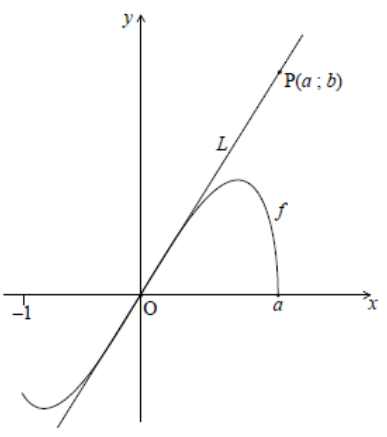
\includegraphics[scale=0.3]{temp_2xsqrtasq-xsq}\par
  \end{center}
  \medskip
  \noindent La droite $L$ est la tangente à la représentation graphique de $f$ à l'origine, $O$.\par
  \noindent Le Point $P(a; b)$ est sur $L$.\par
  \medskip
  (a)\par
  \hspace{1em}(i)  Étant donné que $f^\prime(x) =\frac{2a^2 - 4x^2}{\sqrt{a^2-x^2}}$, pour $-1 \le x \le a$,\par
  \hspace{2em} trouvez l'équation de $L$.\par
  \medskip
  \hspace{1em}(ii) À partir de là ou par toute autre methode, trouvez in l'expression pour $b$ en fonction de $a$\hspace*{\fill} [16]\par
  \medskip
  
\end{question}

%7
\bigskip
\begin{question}
  \hspace*{\fill} [Note maximale: 16]\par
  \medskip
  \noindent La figure suivante représente une partie de la représentation graphique de la fonction $f(x) = 2x^2$.\par
  \medskip
  \begin{center}
    \noindent La figure n'est pas a l'échelle\par
    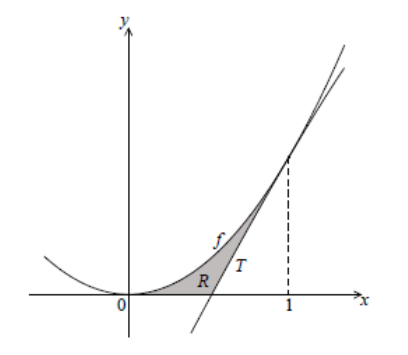
\includegraphics[scale=0.4]{temp_f_2xsquared}\par
  \end{center}
  \medskip
  \noindent La droite T est la tangente à la représentation graphique de $f$ en $x = 1$.\par
  \medskip
  (a) Montrez que l’équation de $T$ est $y = 4x - 2$.\hspace*{\fill} [5]\par
  \medskip
  (b) Trouvez l’abscisse à l’origine de $T$.\hspace*{\fill} [2]\par
  \medskip
  (c) La région grisée $R$ est limitée par la représentation graphique de $f$, la droite $T$ et l’axe des abscisses.\par
  \hspace{1em}(i)  Donnez une expression de l’aire de $R$.\par
  \hspace{1em}(ii) Trouvez l’aire de $R$.\hspace*{\fill} [9]\par
  \medskip
\end{question}
\newpage
%8
\begin{question}
  \hspace*{\fill} [Note maximale: 15]\par
  \medskip
  \noindent La figure suivante représente une partie de la représentation graphique de la fonction quadratique $f$.\par
  \medskip
  \begin{center}
    % \noindent La figure n'est pas a l'échelle\par
    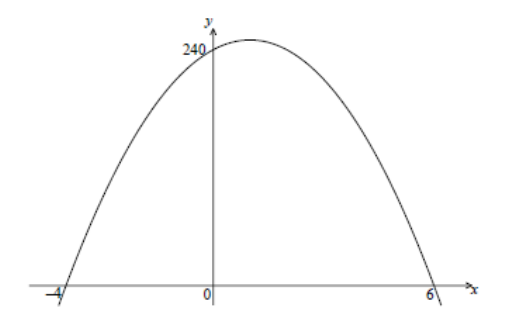
\includegraphics[scale=0.3]{temp_down_parabola}\par
  \end{center}
  \medskip
  \noindent Les abscisses à l’origine sont en (-4; 0 ) et (6; 0) et l’ordonnée à l’origine est en (0; 240).\par
  \medskip
  (a) Donnez $f(x)$ sous la forme $f(x) = -10(x - p) (x - q)$.\hspace*{\fill} [2]\par
  \medskip
  (b) Trouvez une autre expression de $f(x)$ sous la forme $f(x) = -10(x - h)^2 + k$.\hspace*{\fill} [4]\par
  \medskip
  (c) Montrez que $f(x)$ peut aussi s’écrire sous la forme $f(x) = 240 + 20x -10x^2$.\hspace*{\fill} [2]\par
  \medskip
  \noindent Une particule se déplace en ligne droite de telle sorte que sa vitesse $v$ (en $ms^{-1}$ ),
au temps $t$ (en secondes), est donnée par $v = 240 + 20t -10t^2$ , avec $0 \le t \le 6$\par
  (d)\par
  \medskip
  \hspace{1em}(i)  Trouvez la valeur de $t$ quand la vitesse de la particule est la plus grande.\par
  \hspace{1em}(ii) Trouvez l’accélération de la particule quand sa vitesse est nulle.\hspace*{\fill} [7]\par
\end{question}
%9
\bigskip
\begin{question}
  \hspace*{\fill} [Note maximale: 6]\par
  \medskip
  \noindent Soit $f(x) = kx^4$. Le point $P(1 ; k)$ est sur la courbe représentant $f$. En $P$, la normale à la courbe est parallèle à $y = -\frac{1}{8}x$.\par
  \medskip
  Trouvez la valeur de $k$.\hspace*{\fill} [6]\par
\end{question}

%10
\bigskip
\begin{question}
  \hspace*{\fill} [Note maximale: 6]\par
  \noindent Une fonction $f$ est définie pour $-4 \le x \le 3$. La représentation graphique de $f$ est donnée ci-dessous.\par
  \medskip
  \begin{center}
    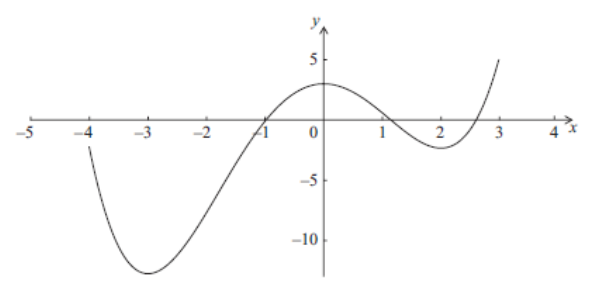
\includegraphics[scale=0.25]{temp_polynom_minus4_to_3}\par
  \end{center}
  \noindent La représentation graphique présente un maximum relatif en $x = 0$ et des minimums relatifs en $x = -3$ et $x = 2$.\par
  \medskip
  (a) Donnez les abscisses à l’origine de la représentation graphique de la fonction dérivée, $f^\prime$.\hspace*{\fill} [2]\par
  \medskip
  (b) Donnez toutes les valeurs de $x$ pour les quelles $f^\prime(x)$ est positive.\hspace*{\fill} [2]\par
  \medskip
  (c) Au point $D$ sur la représentation graphique de $f$, l’abscisse est $-0,5$.\par
  \hspace{2em} Expliquez pourquoi $f^{\prime\prime}(x) < 0$ en $D$.\hspace*{\fill} [2]\par
\end{question}
\newpage
%11
\begin{question}
  \hspace*{\fill} [Note maximale: 14]\par
  \medskip
  \noindent On considère la fonction $f$ dont la dérivée seconde est $f^{\prime\prime}(x) = 3x -1$. La représentation graphique de $f$ présente un point minimum en $A(2 ; 4)$ et un point maximum en $B(-\frac{4}{3}; \frac{358}{27})$.\par
  \medskip
  (a) Utilisez la dérivée seconde pour justifier que $B$ est un maximum.\hspace*{\fill} [3]\par
  \medskip
  (b) Étant donné que $f^\prime(x) = \frac{3}{2}x^2 - x + p$, montrez que $p = -4$.\hspace*{\fill} [4]\par
  \medskip
  (c) Trouvez $f(x)$.\hspace*{\fill} [7]\par
\end{question}
\bigskip
%12
\begin{question}
  \hspace*{\fill} [Note maximale: 17]\par
  \medskip
  \noindent Soit $f(x) = 6 + 6$ sin $x$. Une partie de la representation grafique the $f$ est donnée ci-dessous.\par
  \medskip
  \begin{center}
    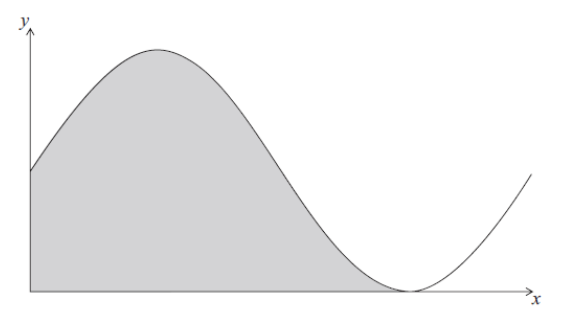
\includegraphics[scale=0.3]{temp_6_plus_6sinx}\par
  \end{center}
  \medskip
  \noindent La région grisée est limitée par la courbe représentant $f$, l’axe des abscisses et l’axe des ordonnées.\par
  \medskip
  (a) Resolvez, avec $0 \le x \le 2\pi$\par
  \hspace{1em} (i ) $6$ + sin $x = 6$;\par
  \hspace{1em} (ii) $6$ + sin $x = 0$.\hspace*{\fill} [5]\par
  \medskip
  (b) Donnez la valeur exacte de l’abscisse à l’origine de $f$, avec $0 \le x \le 2\pi$.\hspace*{\fill} [1]\par
  \medskip
  (c) L’aire de la région grisée est $k$. Trouvez la valeur de $k$, en donnant votre réponse en fonction de $\pi$.\hspace*{\fill} [6]\par
  \medskip
  \noindent Soit $g(x) = 6 + 6$ sin $(x - \frac{\pi}{2})$. La representation graphique the $f$ est transformeé en celle de $g$.\par
  \medskip
  (d) Donnez une description géométrique complète de cette transformation.\hspace*{\fill} [2]\par
  \medskip
  (e) Étant donné que $\int_p^{p+\frac{3\pi}{2}}g(x)\,dx =k$ et $0 \le p < 2\pi$, donnez les deux valeur de $p$.\hspace*{\fill} [3]\par
\end{question}

%13
\bigskip
\begin{question}
  \hspace*{\fill} [Note maximale: TBD]\par
  \medskip
  \noindent Soit $f^\prime(x) = 12x^2 - 2$.  Sachant que $f(-1) = -1$, trouvez $f(x)$.\hspace*{\fill} [TBD]\par
\end{question}

%14
\bigskip
\begin{question}
  \hspace*{\fill} [Note maximale: TBD]\par
  \medskip
  \noindent La vitesse $v$, en $ms^{-1}$, d’une particule se déplaçant en ligne droite est donnée par $v=e^{3t-2}$, ou $t$ est le temps en secondes.\par
  \medskip
  (a) Trouvez l’accélération de la particule à l’instant $t = 1$.\hspace*{\fill} [TBD]\par
  \medskip
  (b) Pour quelle valeur de $t$ la particule a-t-elle une vitesse de $22,3ms^{-1}$?\hspace*{\fill} [TBD]\par
  \medskip
  (c) Trouvez la distance parcourue pendant la première seconde.\hspace*{\fill} [TBD]\par
\end{question}
%15
\begin{question}
  \hspace*{\fill} [Note maximale: TBD]\par
  \medskip
  \noindent Soit $f(x) = 3 Cos2x + Sin^2x$.\par
  \medskip
  (a) Montrez que $f^\prime(x) = -5Sin2x$.\hspace*{\fill} [TBD]\par
  \medskip
  (b) Dans l'intervalle $\frac{\pi}{4} \le x \le \frac{3\pi}{4}$,\par
  \hspace{1em} une normale à la représentation graphique de $f$ a pour équation $ x = k $.\par
  \hspace{1em} Trouvez la valeur de $k$. \hspace*{\fill} [TBD]\par
  \medskip
\end{question}
\section*{\textbf{Calculatrice Graphique Permise}}

%16
\begin{question}
  \hspace*{\fill} [Note maximale: 15]\par
  \medskip
  \noindent Une particule $P$ se déplace le long d’une droite. Le vecteur vitesse $v$ $ms^{-1}$ de $P$ après $t$ secondes est donnée par $v(t) = 7 cos t - 5t^{cos t}$, pour $0 \le t \le 7$. Le diagramme suivant montre la représentation graphique de $v$.\par
  \medskip
  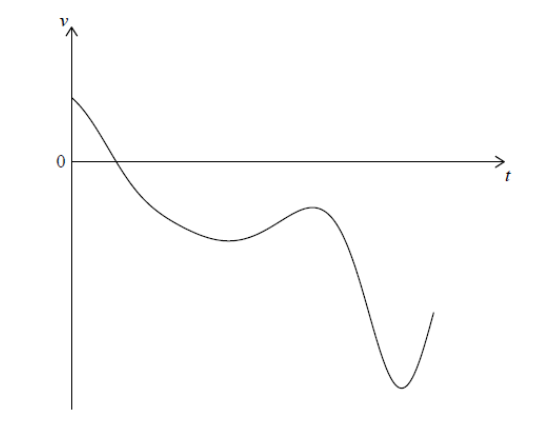
\includegraphics[scale=0.3]{temp_graph_v_vs_t}\par
  \medskip
  (a) Trouvez le vecteur vitesse initiale de $P$.\hspace*{\fill} [2]\par
  \medskip
  (b) Trouvez la vitesse maximale de $P$.\hspace*{\fill} [3]\par
  \medskip
  (c) Écrivez le nombre de fois où l’accélération de $P$ est $0$ $ms^{-2}.$\hspace*{\fill} [3]\par
  \medskip
  (d) Trouvez l’accélération de $P$ lorsque la particule change de direction.\hspace*{\fill} [4]\par
  \medskip
  (e) Trouvez la distance totale parcourue par $P$.\hspace*{\fill} [3]\par
\end{question}
%17
\bigskip
\begin{question}
  \hspace*{\fill} [Note maximale: 6]\par
  \medskip
  \noindent Soit $f(x) = Cos(e^x)$, pour $-2 \le x \le 2$.\par
  \medskip
  (a) Trouvez $f^\prime(x)$.\hspace*{\fill} [TBD]\par
  \medskip
  (b) Sur le système d'axes ci-dessous, esquissez la représentation graphique de $f^\prime(x)$.\hspace*{\fill} [TBD]\par
  \medskip
  \begin{flushleft}
    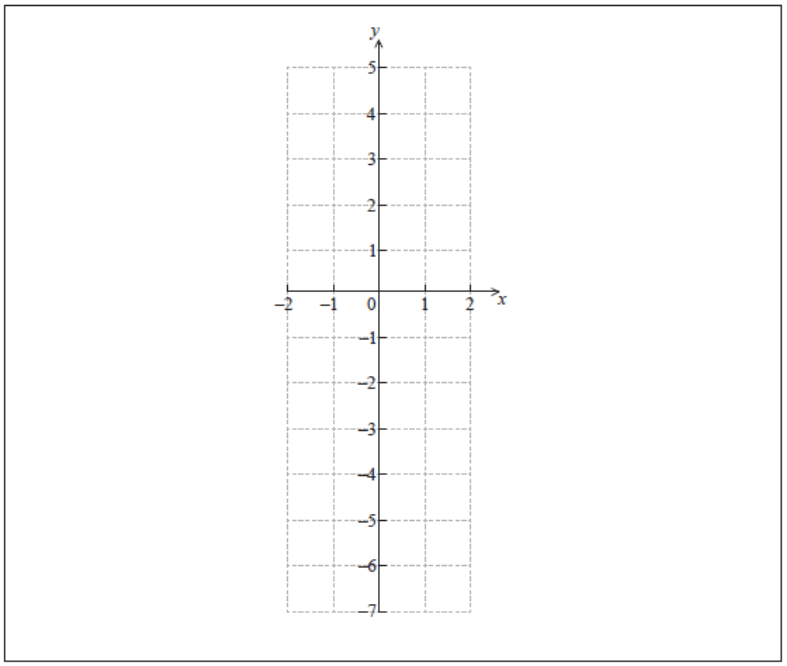
\includegraphics[scale=0.3]{grid_5_12}\par
  \end{flushleft}
\end{question}

%18
\bigskip
\begin{question}
  \hspace*{\fill} [Note maximale: 6]\par
  \medskip
  \noindent Une particule se déplace sur une ligne droite avec une vitesse $v = 12t - 2t^3 - 1$, pour $t \ge 0$, oú $v$ est en centimetres par seconde et $t$ est en secondes.\par
  \medskip
  (a) Trouvez l’accélération de la particule à l’instant $t = 2,7$ secondes.\hspace*{\fill} [3]\par
  \medskip
  (b) Trouvez le déplacement de la particule apres $1,3$ secondes.\hspace*{\fill} [3]\par
\end{question}

%19
\newpage
\begin{question}
  \hspace*{\fill} [Note maximale: 13]\par
  \medskip
  \noindent Soit $f(x) = ax^3 + bx^2 + c$, ou $a$, $b$ et $c$ sont des nombres reéls. La courbe de $f$ passe par le point $(2;9)$.\par
  \medskip
  (a) Montrez que $8a + 4b +c = 9$ .\hspace*{\fill} [2]\par
  \medskip
  \noindent La courbe de $f$ a un minimum relativ en $(1; 4)$.\par
  \medskip
  (b) Trouvez deux autres équations en termes de $a$ , $b$ et $c$, en donnant vos réponses sous\par
  \hspace{1em} une forme similaire à celle de la partie (a).\hspace*{\fill} [7]\par
  (c) Trouvez la valeur de $a$, celle de $b$ et celle de $c$.\hspace*{\fill} [4]\par
\end{question}

%20
\bigskip
\begin{question}
  \hspace*{\fill} [Note maximale: 8]\par
  \medskip
  \noindent La pente d’une fonction est donnée par $\dfrac{dy}{dx} = 10e^{2x - 5}$. Quand $x = 0$ et $y = 8$.\par
  \medskip
  \noindent Trouvez la valeur de $y$  quand $x = 1$.\hspace*{\fill} [8]\par
\end{question}

%21
\bigskip
\begin{question}
  \hspace*{\fill} [Note maximale: 6]\par
  \noindent Soit $f(x) = e^x Sin 2x + 10$, avec $0 \le x \le  4$.  Une partie de la représentation graphique de $f$ est donnée ci-dessous.\par
  \medskip
  \begin{center}
    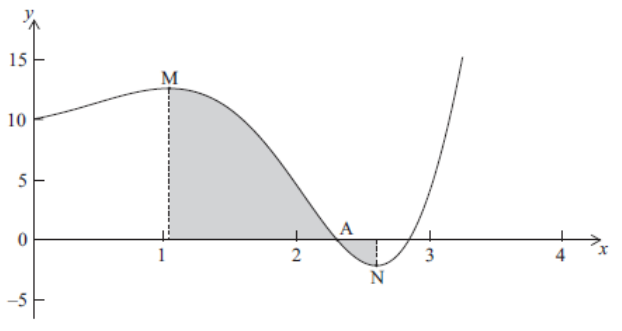
\includegraphics[scale=0.25]{etox_sin2x}\par
  \end{center}
  \noindent Sont représentés une abscisse a l'origine au point $A$, un maximum relatif au point $M$ avec $x = p$ et un minimum relatif au point $N$ avec $x = q$.\par
  \medskip
  (a) Donnez les abscisses de $A$.\hspace*{\fill} [1]\par
  \medskip
  (b) Trouvez la valeur de\par
  \hspace{1em} (i ) $p$\par 
  \hspace{1em} (ii) $q$\hspace*{\fill} [2]\par
  \medskip
  (c) Trouvez $\int_p^qf(x)dx$. Expliquez pourquoi ceci n'est pas l'aire de la région grisée.\hspace*{\fill} [3]\par

  
\end{question}

%22
\newpage
\begin{question}
  \hspace*{\fill} [Note maximale: 14]\par
  \noindent On considère $f(x) = x\ln(4 - x^2)$, avec $-2 < x < 2$.\par
  \medskip
  \begin{center}
    \noindent Une partie de la représentation graphique de $f$ est donnée ci-dessous.\par
    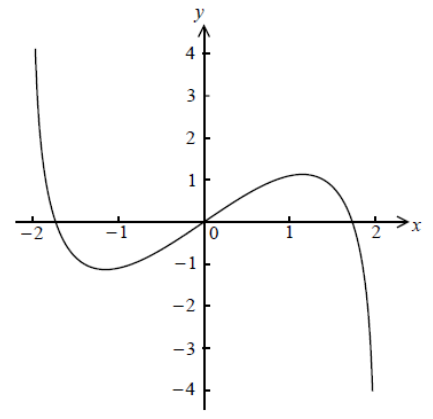
\includegraphics[scale=0.25]{xln4minuxsqr}\par
  \end{center}\par
  (a) Soient $P$ et $Q$ les points de la courbe représentant $f$\par
  \hspace{1em} où la tangente à la représentante graphique de $f$ est parallèle à l'axe des abscisses.\par
  \hspace{1em} (i ) Trouvez l'abscisse de $p$ et $q$.\par 
  \hspace{1em} (ii) On considère $f(x) =k$.\par
  \hspace{3em} Donnez toutes les valeurs de $k$ pour les-quelles il y a exactement deux solutions.\hspace*{\fill} [5]\par
  \medskip
  Soit $g(x) = x^3\ln(4 - x^2)$, avec $-2 < x < 2$.\par
  \medskip
  (b) Montrez que $g^\prime(x)=\frac{-2x^4}{4 - x^2} + 3x^2\ln(4 - x^2)$.\hspace*{\fill} [4]\par
  \medskip
  (c) Esquissez la représentation graphique de $g^\prime$.\hspace*{\fill} [2]\par
  \medskip
  (d) On considére $g^\prime(x) = w$.\par
  \hspace{1em} Donnez toutes les valeurs de $w$ pour les-quelles il y a exactement deux solutions.\hspace*{\fill} [3]\par

  
  
\end{question}

\end{document}
